\chapter{Resultaten Experimenten}
In dit hoofdstuk gaan we kijken hoe de risicobeperkende maatregelen de performantie van verschillende webservices beïnvloeden.
Het vergelijken wordt vooraf gegaan door een t-test, die duidelijk zal maken of het verschil statistisch significant is. Hiervoor wordt de alpha-waarde als standaard genomen: 0,05. De p-waarde moet kleiner zijn als de alpha-waarde, om met zekerheid te zeggen dat de meetresultaten betrouwbaar zijn.

\section{CPU gebruik}
De belasting werd gegenereerd door autobench met 40 verzoeken per seconde voor een totaal van 4500 verzoeken.
Het CPU gebruik werd opgeslaan elke seconde voor 90 seconden met vmstat.
Het vmstat commando wordt naar de webservers gedelegeerd.


\begin{figure}
	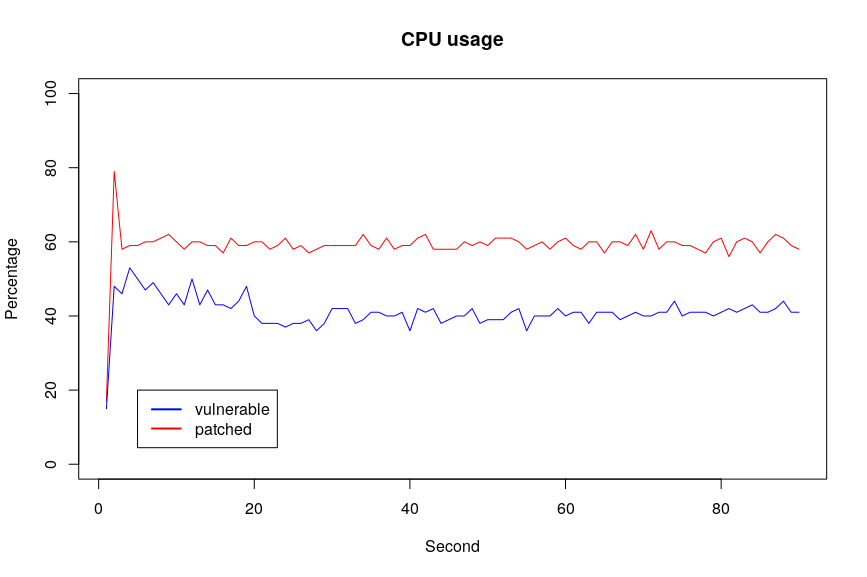
\includegraphics[width=1.0\linewidth]{img/cpu_usage.png}
	\caption{CPU gebruik}
	\label{fig:cpu_usage}
\end{figure}

\begin{figure}
	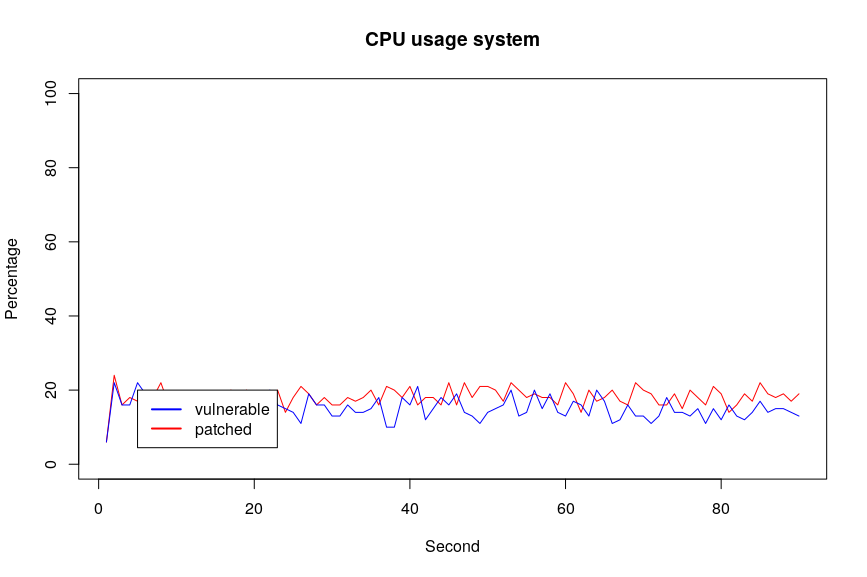
\includegraphics[width=1.0\linewidth]{img/cpu_system.png}
	\caption{CPU gebruik kernelspace}
	\label{fig:cpu_system}
\end{figure}

\begin{figure}
	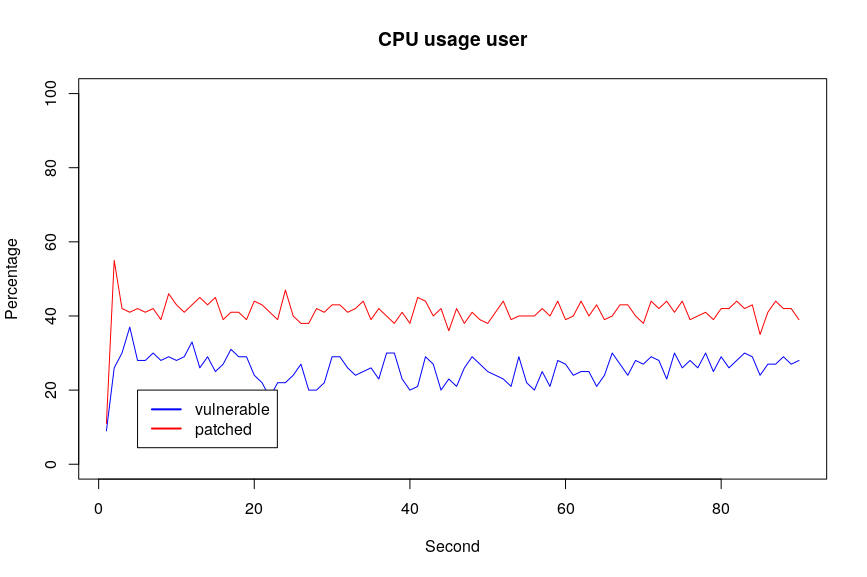
\includegraphics[width=1.0\linewidth]{img/cpu_user.png}
	\caption{CPU gebruik userspace}
	\label{fig:cpu_user}
\end{figure}

\begin{table}[]
	\centering
	\caption{t-test voor cpu gebruik}
	\label{t_cpu}
\begin{tabular}{l|rr}
	\hline
	patch              & \multicolumn{1}{c}{MET} & \multicolumn{1}{c}{ZONDER} \\
	gemiddelde         & 59.13\%                 & 41.10\%                    \\
	standaard deviatie & 5.13\%                  & 4.21\%                     \\
	aantal resultaten  & 90                      & 90                         \\ \hline
	p-waarde           & \multicolumn{2}{c|}{2.2e-16}                        
\end{tabular}


\end{table}

\begin{table}[]
	\centering
	\caption{t-test voor cpu gebruik gebruikersruimte}
	\label{t_cpu_us}
	\begin{tabular}{l|rr}
		\hline
		patch              & \multicolumn{1}{c}{MET} & \multicolumn{1}{c}{ZONDER} \\
		gemiddelde         & 47.10\%                 & 25.88\%                    \\
		standaard deviatie & 4.16\%                  & 3.85\%                     \\
		aantal resultaten  & 90                      & 90                         \\ \hline
		p-waarde           & \multicolumn{2}{c|}{2.2e-16}                        
	\end{tabular}
\end{table}


\begin{table}[]
	\centering
	\caption{t-test voor cpu gebruik kernelruimte}
	\label{t_cpu_sys}
	\begin{tabular}{l|rr}
		\hline
		patch              & \multicolumn{1}{c}{MET} & \multicolumn{1}{c}{ZONDER} \\
		gemiddelde         & 18.06\%                 & 15.22\%                    \\
		standaard deviatie & 2.51\%                  & 2.92\%                     \\
		aantal resultaten  & 90                      & 90                         \\ \hline
		p-waarde           & \multicolumn{2}{c|}{5.983e-11}                      
	\end{tabular}
\end{table}


De grafiek op figuur \ref{fig:cpu_usage} is berekend met het vmstat commando.

Elke seconde slaat vmstat het processor gebruik op voor zowel 'user CPU' en 'sys CPU'.
Het verschil is of de applicatie tijd heeft doorgebracht in gebruikersruimte (user space) of kernelruimte (kernel space).
Systeemtijd (system calls) is tijd besteed aan het uitvoeren van code in de kernel van het besturingssysteem namens de applicatie.

Het gemiddelde van het ongepatchte systeem is 41,10\%, het gemiddelde van het gepatchte systeem is 59,13\%. Dit is een stijging van 43,87\%.

Het verbruik in gebruikersruimte is gestegen van 25,88\% naar 41,08\%, een stijging van 58,73\%(figuur \ref{fig:cpu_user}).

Het verbruik in kernelruimte is gestegen van 15,22\% naar 18,06\%, een stijging van 18,66\%(figuur \ref{fig:cpu_system}).

Met de retpoline patch heeft dit systeem veel moeite. Branch prediction speelt een grote rol op deze CPU.

Het is dus duidelijk te zien dat overgangen van gebruikersruimte naar kernelruimte meer lijden onder de patches.
Herinner wel dat het effect wordt verergerd door de hypervisor van virtualbox.


Elke p-waarde is kleiner dan de corresponderende alpha-waarde (0,05), er is dus bij elke test een statistisch
significant verschil gevonden.







\section{Responstijd}

\begin{figure}
	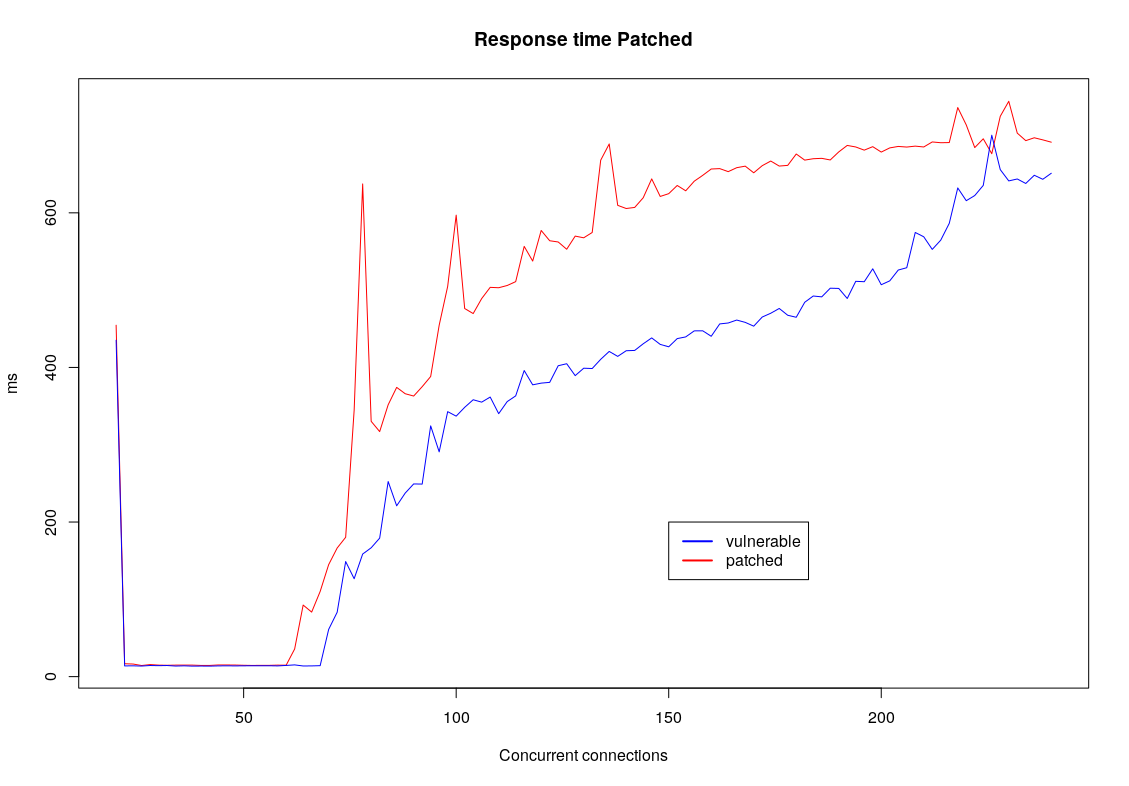
\includegraphics[width=1.0\linewidth]{img/ms_conc.png}
	\caption{Latentie tot 240 gelijktijdige verbindingen}
	\label{fig:ms_conc}
\end{figure}

\begin{figure}
	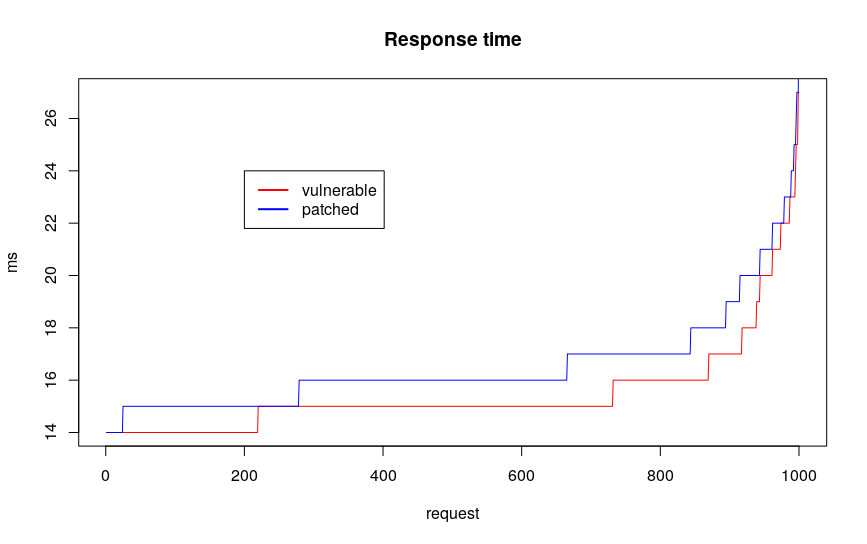
\includegraphics[width=1.0\linewidth]{img/ms_patched_vuln.png}
	\caption{Latentie tot 1000 verzoeken}
	\label{fig:ms_patched_vuln}
\end{figure}

\begin{table}[]
	\centering
	\caption{t-test voor latentie tot 240 gelijktijdige verbindingen}
	\label{t_ms_conc}
	\begin{tabular}{l|cr}
		\hline
		patch              & MET                        & \multicolumn{1}{c}{ZONDER} \\
		gemiddelde         & \multicolumn{1}{r}{466.02} & 342.61                     \\
		standaard deviatie & \multicolumn{1}{r}{261.29} & 212.37                     \\ \hline
		p-waarde           & \multicolumn{2}{c|}{0.0001499}                         
	\end{tabular}
\end{table}

\begin{table}[]
	\centering
	\caption{t-test voor latentie tot 1000 verzoeken}
	\label{t_ms_patched_vuln}
	\begin{tabular}{l|cr}
		\hline
		patch              & MET                       & \multicolumn{1}{c}{ZONDER} \\
		gemiddelde         & \multicolumn{1}{r}{15.62} & 14.77                      \\
		standaard deviatie & \multicolumn{1}{r}{1.53}  & 1.74                       \\ \hline
		p-waarde           & \multicolumn{2}{c|}{2.2e-16}                          
	\end{tabular}
\end{table}


Figuur \ref{fig:ms_conc} werd verkregen door de latentie te berekenen voor een bepaald aantal van gelijktijdige verbindingen.

De gelijktijdige verbindingen lopen uiteen van 20 tot 240 met stappen van 2. 
De gebruikte tool heet 'autobench'.

Een voordeel van het geleidelijk aan, simultane verbindingen kunnen verzenden, is dat er geen onafhankelijke tests moeten uitgevoerd worden voor het breekpunt te bepalen.
Deze probleemoplossende strategie wordt 'guess-and-check tests' genoemd.
Deze methode neemt veel tijd in beslag en is zeer omslachtig.
Maar de kans is ook groot dat de resultaten niet weergeven of de applicatie ongunstig reageert.

Jakob Nielsen heeft onderzocht wat een aanvaardbare responstijd is voor elke toepassing (websites zijn in dit opzicht niet speciaal).
Nielsens zegt dat 0,1 seconde ongeveer het limiet is om de gebruiker het gevoel te geven dat het systeem onmiddellijk reageert, één seconde is ongeveer de limiet voor de gedachtestroom van de gebruiker om ononderbroken te blijven, ook al merkt de gebruiker de vertraging op.
En tien seconden is ongeveer de limiet om de aandacht van de gebruiker gericht te houden \parencite{Nielsen1993}.

Het systeem met patches kan 66 gelijktijdige verbindingen aan voor een responstijd van minder dan 0,1 seconde.
Het systeem zonder patches kan 72 gelijktijdige verbindingen aan.
De p-waarde van de resultaten zijn 0,0001499, dus het resultaat is statistisch betrouwbaar.


De resultaten van figuur \ref{fig:ms_patched_vuln} werden gemaakt met de Apache HTTP server benchmarking tool (ab).

Het gemiddelde van het systeem met de patches is 15,62 milliseconden, van het systeem zonder patches is het 14,77, een verschil van 5\%.
De p-waarde is ruim onder de 5\%.


\section{Redis}

\begin{figure}
	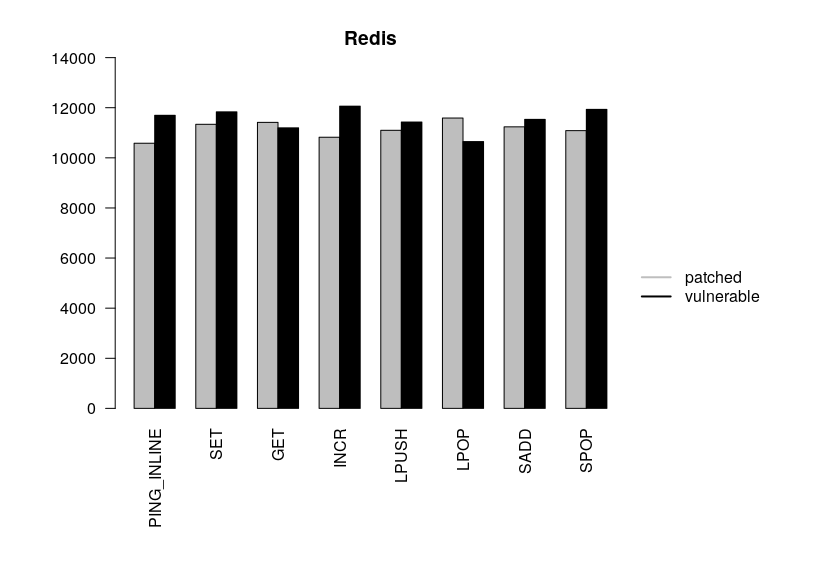
\includegraphics[width=1.0\linewidth]{img/redis.png}
	\caption{Redis}
	\label{fig:redis}
\end{figure}

\begin{table}[]
	\centering
	\caption{t-test voor redis}
	\label{t_redis}
	\begin{tabular}{l|cr}
		\hline
		patch              & MET                          & \multicolumn{1}{c}{ZONDER} \\
		gemiddelde         & \multicolumn{1}{r}{11145.83} & 11542.07                   \\
		standaard deviatie & \multicolumn{1}{r}{325.3505} & 456.8148                   \\ \hline
		p-waarde           & \multicolumn{2}{c|}{0.06764}                             
	\end{tabular}
\end{table}


De resultaten van redis (figuur \ref{fig:redis} ) zijn berekend met 'redis-benchmark', een hulpprogramma opgenomen in Redis.

Het systeem met patches verliest 3,4\% performantie.
Helaas is de p-waarde (tabel \ref{t_redis}) net niet laag genoeg om met zekerheid te zeggen dat de resultaten betekenisvol zijn.




\section{Doorvoersnelheid}

\begin{figure}
	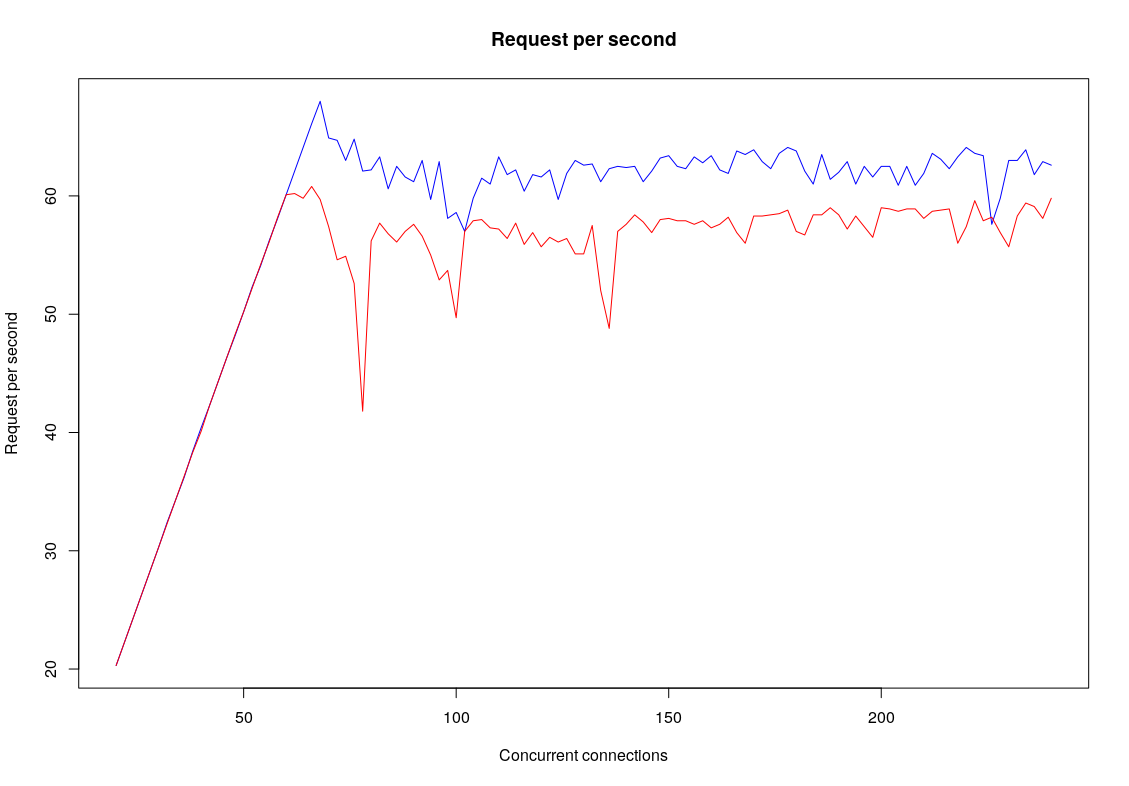
\includegraphics[width=1.0\linewidth]{img/rps.png}
	\caption{Doorvoersnelheid}
	\label{fig:rps}
\end{figure}

\begin{table}[]
	\centering
	\caption{t-test voor doorvoersnelheid}
	\label{t_rps}
	\begin{tabular}{l|cr}
		\hline
		patch              & MET                          & \multicolumn{1}{c}{ZONDER} \\
		gemiddelde         & \multicolumn{1}{r}{53.87297} & 58.16126                   \\
		standaard deviatie & \multicolumn{1}{r}{8.76}     & 10.26                      \\ \hline
		p-waarde           & \multicolumn{2}{c|}{0.0009614}                           
	\end{tabular}
\end{table}

De doorvoersnelheid werd met dezelfde methode berekend als de responstijd (20 tot 240 gelijktijdige verbindingen met stappen van 2).

Het systeem met de patches heeft een doorvoersnelheid van 54 verzoeken per seconde, het systeem zonder patches een doorvoersnelheid van 58 (figuur \ref{fig:rps}).
Dit is een verlies van 7 procent.
